
\documentclass[aspectratio=169]{beamer}
% metadata
\title{Nonnegative Matrix Factorization}
\subtitle{Be Positive!}
\author{Abdelbast Nassiri \\ Maximilian Stollmayer \\ Manuel Wissiak}
\institute{University of Vienna}
\date{30.01.2023}

% \usetheme[titlestyle=plain, sectionstyle=style1, slidestyle=style1]{trigon}
% \usepackage{amsmath}
% \usepackage{amssymb}
% \usepackage{hyperref}
% \usepackage{setspace}
% \usepackage{xpatch}
% \usepackage{lipsum}
% \usepackage{tcolorbox}
% \usepackage{graphicx}
% \tcbuselibrary{fitting}
% \hypersetup{
%     colorlinks=true,
%     linkcolor=blue,
%     filecolor=magenta,      
%     urlcolor=cyan,
%     pdftitle={Overleaf Example},
%     pdfpagemode=FullScreen,
%     }
% 
% \RestyleAlgo{ruled}
% % \usepackage{algorithm}
% % \usepackage{algorithmic}
% % \usepackage{pseudocode}
% % \usepackage{float}
% \makeatletter
% \patchcmd\beamer@@tmpl@frametitle{\insertframetitle}{\insertsection\space-- \insertframetitle}{}{}
% \makeatother

% theme
\usetheme[titlestyle=plain, sectionstyle=style1, slidestyle=style1]{trigon}

% packages
\usepackage{multicol} % for two columns in algorithms section
    \setlength{\columnseprule}{1pt}
    \setlength{\columnsep}{1cm}
\usepackage{amsmath}
\usepackage{mathtools}
\usepackage{algorithm2e}
\usepackage{optidef}
\usepackage{epigraph}
\usepackage{array}


\begin{document}

% title ------------------------------------------------------------------------
\titleframe

% Manuel ----------------------------------------------------------------------
% https://citeseerx.ist.psu.edu/document?repid=rep1&type=pdf&doi=8116d41cb547671bb9c38ffe47574e5cdf24fa7e
% https://ar5iv.labs.arxiv.org/html/1401.5226
% https://ar5iv.labs.arxiv.org/html/1703.00663
% https://ar5iv.labs.arxiv.org/html/0708.4149

\begin{frame}{NMF}
    \begin{block}{Problem}
        Given \(A \in \mathbb{R}^{m \times n}_+\) non-negative and \emph{rank} \(r \leq \min(m, n)\). \\
        Find \(W \in \mathbb{R}^{m \times r}_+\) and \(H \in \mathbb{R}^{r \times n}_+\) both non-negative s.t.: \\
        \[A \approx WH\]
    \end{block}
\end{frame}

\begin{frame}{Text Mining}
    "Words which are similar in meaning occur in similar contexts"
    \begin{center}
    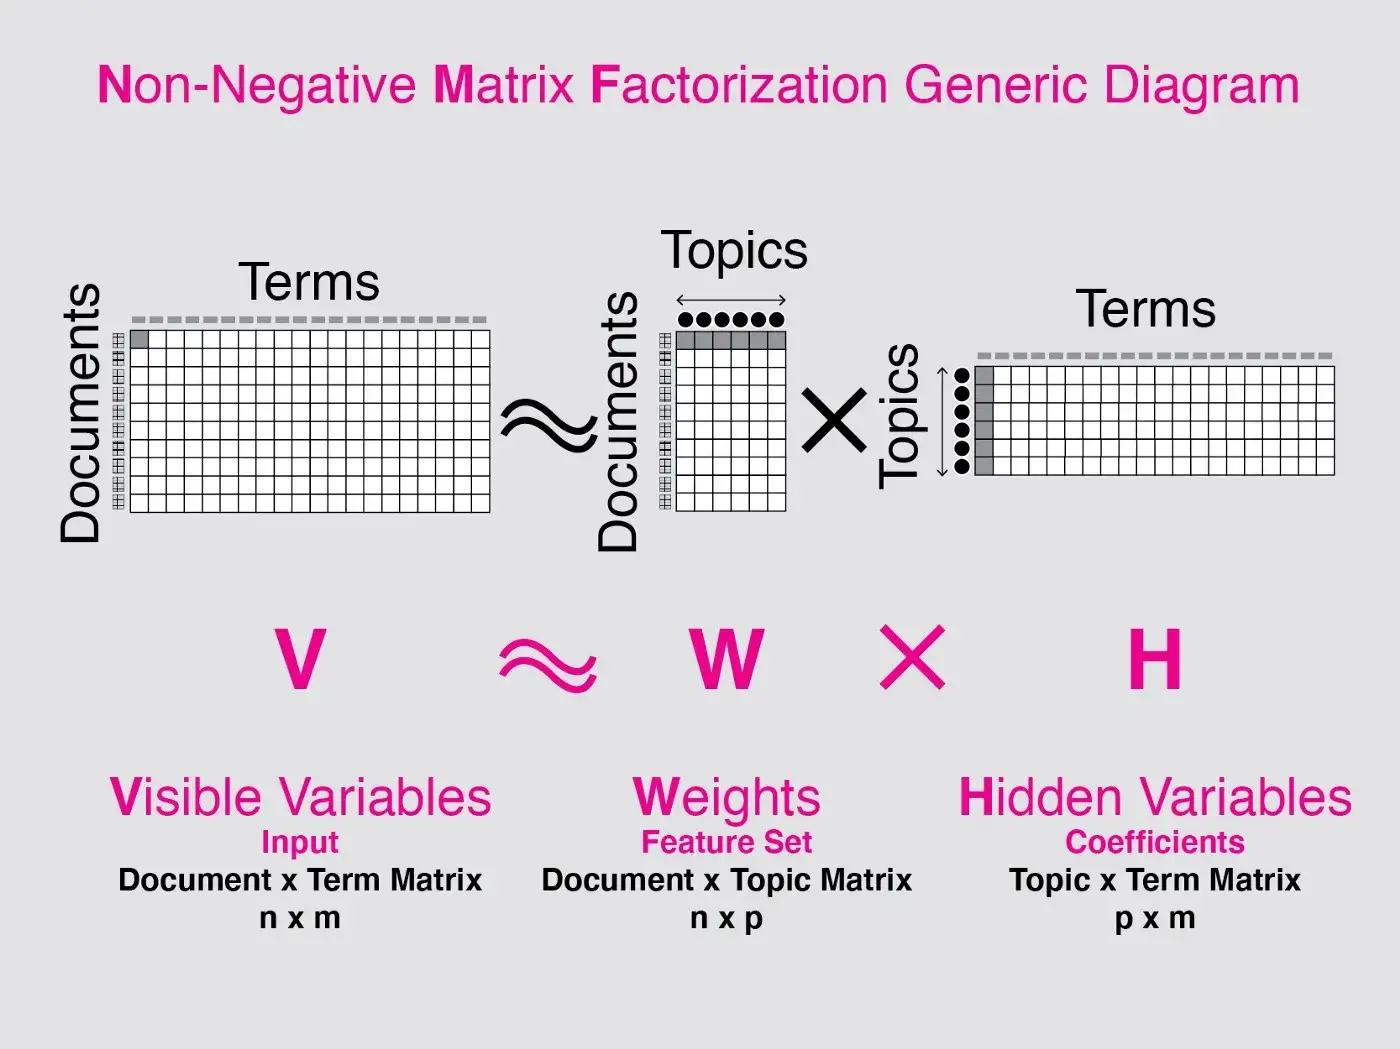
\includegraphics[height = 2in, width = 3.4in]{textmine.png} \\
    \source{Source: "NMF — A visual explainer and Python Implementation", Anupama Garla}    
    \end{center}
\end{frame}

\begin{frame}{Image Processing}
    Given vectorized gray-levels \(X \in \mathbb{R}^{p \times n}_+\) of $n$ facial images. \\
    Problem: Facial Feature Extraction
    \begin{center}
    \begin{tabular}{ c c l }
     \(X(:,j) \approx \) &  \(\sum_{k=1}^{r} W(:,k) \) & \(H(k,j)\) \\ 
     j-th facial image & facial features & importance of feature in j-th image 
    \end{tabular}
    \end{center}
     
\end{frame}

\begin{frame}{Hyperspectral Unmixing}
    Given vectorized spectral signature \(X \in \mathbb{R}^{p \times n}_+\) of an image. \\
    Problem: Identify Endmembers (Grass, Stone,...)

    \begin{center}
    \begin{tabular}{ c c l }
     \(X(:,j) \approx \) &  \(\sum_{k=1}^{r} W(:,k) \) & \(H(k,j)\) \\ 
     spectral signature & spectral signature of k-th endmember & abundance of k-th endmember
    \end{tabular}
    \end{center}
      
\end{frame}


\begin{frame}{Hyperspectral Unmixing}
    \begin{center}
        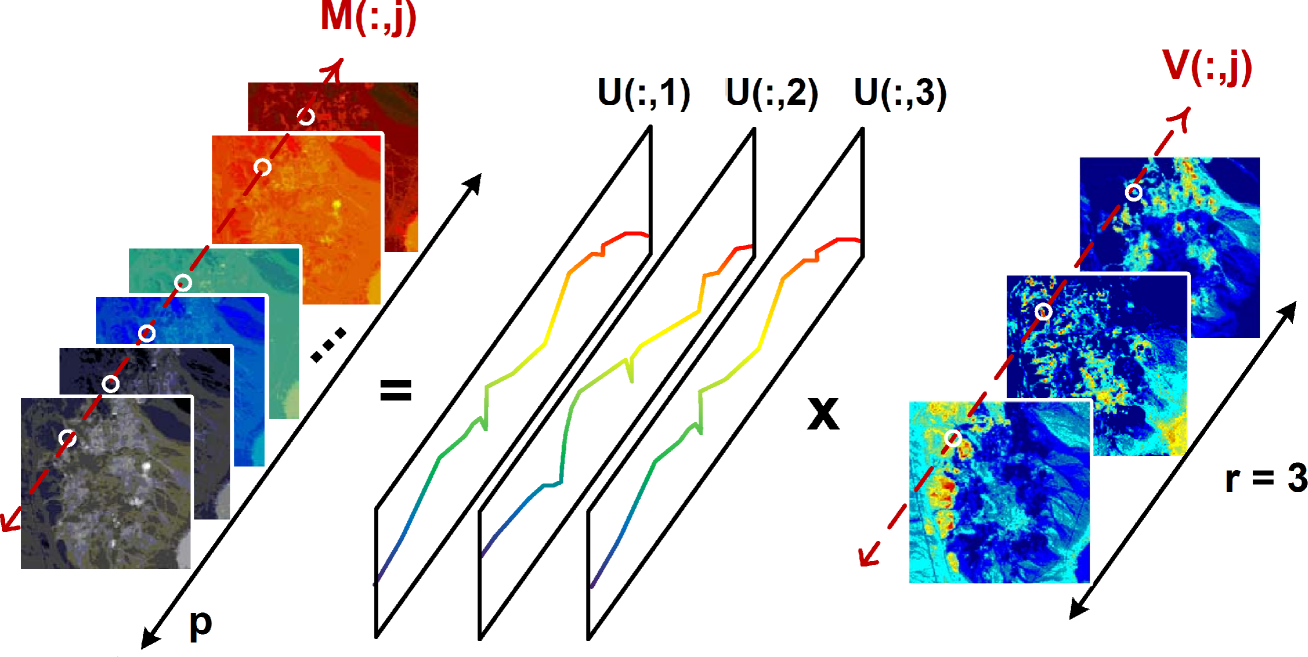
\includegraphics[height = 2.2in, width = 4.4in]{hyperspec.png} \\
        \source{Source: "Introduction to Nonnegative Matrix Factorization", Nicolas Gillis}  
    \end{center}
\end{frame}

\begin{frame}{Problem Reformulation}
    \begin{block}{Optimization Problem}
            Given \(A \in \mathbb{R}^{m \times n}_+\) non-negative and \emph{rank} \(r \leq \min(m, n)\). \\
            \[ \min_{W \in \mathbb{R}^{m \times r}_+, \ H \in \mathbb{R}^{r \times n}_+ } \quad  {\| A - WH \|}_F^2 \]
    \end{block}
    Note that $F(W,H) = {\|A - WH\|}_F^2$ is convex in $U$ and convex in $V$, but not in both!
\end{frame}

\begin{frame}{Stationary Points \& KKT-Conditions}
    % Result of KKT & Stationary
    Checking the KKT-Conditions for \(F(W,H) \) yields the following:
        \[ W \geq 0, \ \nabla_W F = WHH^T - AH^T \geq 0, \ \nabla_W F * W = 0 \]
        \[ H \geq 0, \ \nabla_W F = W^T WH - W^T A \geq 0, \ \nabla_H F * H = 0 \]

    \begin{block}{Stationary Points}
        A pair \((U,V)\) is called a \emph{stationary Point}, if and only if \(U\) and \(V\) satisfy the KKT-Conditions.
    \end{block}
    
\end{frame}

\begin{frame}{Stationary Points \& KKT-Conditions}
    From the KKT-Conditions simple characteristics of the solutions can be derived:
    \begin{block}{Theorem}
        Suppose \( (W,H)\) be a stationary point of the problem, then it holds:
        \[ \frac{1}{2} \|A - WH\|^2 = \frac{1}{2} (\|A\|^2 - \|WH\|^2 )\]
    \end{block}
    This furthermore implies that \( \|A\|^2 \geq \|WH\|^2\), with equality attained only at the exact factoriztion.
\end{frame}

\begin{frame}{Coordinate Descent}
    For $\Omega$ (pointwise) convex \[solve \ \min_{x \in \Omega} f(x) \]
    
    \begin{algorithm}[H]
    \caption{General Coordinate Descent}
        \textbf{Initialization:} \(x \in \mathbb{R}^n\) \\
        \For {$t \gets 1,2, ..., n$} {$solve \ x_i = \underset{\zeta \in \Omega_i}{\arg \min} \ f(x_1, ..., x_{i-1}, \zeta, x_{i+1}, ..., x_n)$}
    \end{algorithm}
\end{frame}

\begin{frame}{"Convergence" Theorem}
    \begin{block}{"Convergence" to stationary Points}
        Suppose $f$ is continuously differentiable and furthermore that \\
        \[\forall i \ \forall x: \min_{\zeta \in \Omega_i} f(x_1, ..., x_{i-1}, \zeta, x_{i+1}, ..., x_n)\] 
        is uniquely attained.
        Let \( \{x^k\} \) be the sequence generated by the \emph{Coordinate Descent}, then every limit point is a stationary point.
    \end{block}
\end{frame}

\begin{frame}{Exact Factorization}
    % nonnegative rank
    Now consider the case where $A$ is exactly factorized by $WH$.
    \begin{block}{minimal rank}
        The smallest $r$ such that exist \(W \in \mathbb{R}^{m \times r}_+ \ and \ H \in \mathbb{R}^{r \times n}_+\) such that $A=WH$, is called the \emph{inner rank} and denoted by $rank_{WH}^+ (A)$. 
    \end{block}

\end{frame}

\begin{frame}{Determining the inner rank}
    One algorithm to determine if $A$ can be factorized with \emph{inner rank} $r$ would be the Renegar algorithm, which scales $(6mn)^{\mathcal{O}(mn)}$. \\
    Since $rank_{WH}^+ (A) \leq \min(m,n)$ this can be done in finite time.
    \begin{block}{Vavasis, 2008}
        \begin{itemize}
            \item exact \emph{NMF} is \emph{NP-hard}
            \item $\exists$ polynomial time local search heuristics
        \end{itemize}
    \end{block}
\end{frame}

% Abdu ------------------------------------------------------------------------
% https://reader.elsevier.com/reader/sd/pii/S0167947306004191?token=F24BE1BF6001274548C15E69DB009E58FA9D3E4D129DF5B97744D22E1D0AA4BE582292713D8FC9C3911BBD86A4CEFA60&originRegion=eu-west-1&originCreation=20230124185843
% https://ieeexplore.ieee.org/stamp/stamp.jsp?tp=&arnumber=6709669

\begin{frame}{Algorithms for NMF}
    \textbf{The Multiplicative Update Rule}
    \begin{align}
        \min_{W,H>0}f(W,H) = \min_{W,H>0} \frac{1}{2}\sum_{i = 1}^{n}\sum_{j= 1}^{m} (A_{ij} - (WH)_{ij})^{2} \label{op}
    \end{align}
    The most used approach to minimize (1) is a simple multiplicative update method
    proposed by Lee and Seung (2001):\\
    This algorithm is just a special case of Gradient Descent with a step size 
    \begin{align*}
        \epsilon(W^{t}) &= \frac{W^{t}}{W^{t}H^{t}(H^{t})^{T}}\\
        \epsilon(H^{t}) &= \frac{H^{t}}{(W^{t})^{T}W^{t}H^{t}}
    \end{align*}
\end{frame}
\begin{frame}{The Multiplicative Update Rule}
\begin{figure}[ht]
  \centering
  \begin{minipage}{.5\linewidth}
    \begin{algorithm}[H]
    \caption{MUR Algorithm}
     \textbf{Initialization:} $W^{1}, H^{1} > 0$\;
    \For {$t \gets 1,2..\dots$} {
    $W^{t+1} = W^{t}\frac{A(H^{t})^{T}}{W^{t}H^{t}(H^{t})^{T}} $\;
    \vspace{0.2in}
    $H^{t+1} = H^{t}\frac{(W^{t+1})^{T}A}{(W^{t+1})^{T}W^{t+1}H^{t}}$\;}
    \end{algorithm} 
    \end{minipage}
    \end{figure}
\end{frame}

\begin{frame}{The Multiplicative Update Rule}
        This algorithm is a type of fixed-point method, meaning that if $(H^{t})^{T} H^{t} W^{t} \neq 0$ and
        $W^{t+1} = W^{t}$, then $A(H^{t})^{T} = W^{t}H^{t}(H^{t})^{T}$ implies 
        $\nabla_{W}f(W^{t}, H^{t}) = 0$,\\
        which is part of the KKT condition.
\end{frame}
\begin{frame}{"Convergence" Theorem}
    \begin{block}{Theorem Lee and Seung}
        -The Euclidean distance $||A - WH||$ is non-increasing under the update rules
        \begin{align*}
            W \gets W\frac{AH^T}{WHH^T}, \hspace{0.3in}
            H \gets H\frac{W^T A}{W^T WH} 
        \end{align*}
        -The Euclidean distance is invariant under these updates if and only if $W$ and $H$ are at
        a stationary point of the distance.
    \end{block}
\end{frame}
\begin{frame}{Weaknesses}
    - Lee and Seung claim that this algorithm "converges" to a stationary point. However, it has been shown in 2005 that this claim is wrong, as having the cost function non-increasing may not imply convergence.\\
    \vspace{0.2in}
    - Therefore, the algorithm still lacks optimization properties.\\
    \end{frame}
    \begin{frame}{Weaknesses}
    - We can only make the following statement about
    the convergence of these algorithms: "When the algorithm has converged to a limit point, this point is a stationary point."\\\
    
    - Also it has been repeatedly shown that the convergence is notoriously slow.
    \end{frame}
    \begin{frame}{Modifications: Convergence vs. speed trade-off}
    - Lin in 2007 proposed a modification that is guaranteed to converge to a stationary point. However, it requires more work per iteration so it is even slower.\\
    \vspace{0.2in}
    - The Fast Multiplicative Update Rule Algorithm from 2014 is faster than the two algorithms in the case of convergence.
\end{frame}

\begin{frame}{Comparison of the the three Algorithms}
    \begin{center}\includegraphics[height = 2.3in]{table.jpg}\end{center}\\
    \source{Source: "A Fast Algorithm for Non-negative Matrix Factorization and Its Convergence", Li, Wu, and Zhang.}
\end{frame}

\begin{frame}{Alternating Non-negative Least Squares (ANLS)}
    - In this algorithms, a least squares step is followed by another least squares step in an alternating fashion, thus giving rise to the ALS name.\\
    - The Alternating Least Squares - ALS algorithms were first introduced by Paatero 1994 , 
    who initially invented the whole NMF Theory.
    \begin{algorithm}[H]
        \caption{Basic ALS for NMF}
        \textbf{Initialization:} $W > 0$\;
        \For {t \gets 1, 2\dots}{
            Solve for H the LS equation $W^{T}WH = W^{T}A$\;
            Set all negative elements in H to 0\;
            Solve for W the LS equation $WHH^{T} = AH^{T}$\;
            Set all negative elements in W to 0\;
        } 
    \end{algorithm}
\end{frame}

\begin{frame}{Convergence Theorem}
    \begin{theorem}
        Any limit point of the sequence $\{W^{t} , H^{t}\}$ generated by ALS Algorithm  is a stationary point.
    \end{theorem}
    \end{frame}
    \begin{frame}{Comparison between ANLS and MU}
\begin{tabular}{|l|l|}
    \hline
    \multicolumn{1}{|c|}{ANLS} & MU \\
    \hline
    + Can be very fast depending on the implementation & + Easy to use  \\
    + Aids sparsity &  \\
    \hline
    -  Once an element in W or H becomes 0, it must remain 0. & - Notoriously slow \\
      & - Lacks optimization properties.\\
    \hline
\end{tabular}   
\end{frame}
\begin{frame}{Comparison between ANLS and MU}
    \includegraphics[height = 2.5in]{comparison.png}\\
    \source{Source: "Fast optimization of non-negative matrix tri-factorization", Zupan, Zitnik}
\end{frame}

\begin{frame}[allowframebreaks]{References}
    \nocite{*}
    \bibliographystyle{plain}
    \bibliography{sources}
\end{frame}

\end{document}
